% Θεμελιώσεις Κρυπτογραφίας 2016
% Εργασία #1
% Κωσταντίνος Σαΐτας - Ζαρκιάς - 2406
% Οδυσσεύς Κρυσταλάκος - 2362
%-------------------------------------------------------------------------

\documentclass[a4paper, 11pt]{article}


\usepackage[english,greek]{babel} % the last language is the default
	\usepackage[utf8x]{inputenc}

%% > UNCOMMENT if your editor uses iso-8859-7 encoding for Greek (typical in Windows System).
% \usepackage[iso-8859-7]{inputenc}

\usepackage{enumerate}
\usepackage{seqsplit}
\usepackage{hyperref}
\usepackage[pdftex]{graphicx}


\newcommand{\lt}{\latintext}
\newcommand{\gt}{\greektext}
\newcommand\tab[1][1cm]{\hspace*{#1}}
%-------------------------------------------------------------------------

\title{Εργασία 1}

\author{Κωσταντίνος Σαΐτας - Ζαρκιάς - 2406 \\ Οδυσσεύς Κρυσταλάκος - 2362}

\date{\today}

%--------------------------------------------------------------------------
\begin{document}

\maketitle

% ===== Θέμα 1 =====
\section*{Θέμα 1}


\begin{itemize}
	\item[{\lt i)}] Η αρχή του {\lt Kerchoff} υποστηρίζει ότι η ασφάλεια ενός κρυπτοσυστήματος δεν πρέπει να βασίζεται στη γνώση του κρυπτοσυστήματος αλλά στη γνώση του μυστικού κλειδιού, δηλαδή σε ένα κρυπτοσύστημα ακόμα και αν είναι ολόκληρη η δομή του γνωστή εκτός από το κλειδί τότε εξακολουθεί να είναι ασφαλές. Η αρχή αυτή έρχεται αντίθετη με την λογική "{\lt security through obscurity}" που στοχεύει στην ασφάλεια του συστήματος κρατώντας την δομή του μυστική που συνεπώς είναι πολύ πιο ευάλωτη στην καταστροφή του. Ένα πρόβλημα που μπορεί να προκύψει με την λογική αυτή είναι ότι αν για κάποιο λόγο σε μία επικοινωνία μαθευτεί η λειτουργία του κρυπτοσυστήματος τότε όλες οι επικοινωνίες που βασίζονταν σε αυτό είναι πλέον ευάλωτες. Αντίθετα, με βάση την αρχή του {\lt Kerchoff} αν μαθευτεί ένα κλειδί μιας επικοινωνίας τότε μόνο αυτή καθιστάται πλέον ευάλωτη ενώ όλες οι υπόλοιπες επικοινωνίες παραμένουν ασφαλής. 
		
	
	
	\item[{\lt ii)}] Ορισμός τέλειας ασφάλειας κατα {\lt Shannon}: Αν κάποιος έχει ολόκληρο το κρυπτογραφημένο μήνυμα {\lt c}, δεν μπορεί να αποκτήσει καμία πληροφορία για το αρχικό μήνυμα {\lt m}.
	
					Ορισμός τέλειας ασφάλειας: Ο ορισμός μπορεί να δωθεί και με ένα υποθετικό παράδειγμα στο οποίο η Αλίκη στέλνει ένα μήνυμα {\lt m0} με τέλεια κρυπτογράφηση στον Μπομπ και δίνει στην Εύα το κρυπτογραφημένο μήνυμα {\lt c}, το αρχικό μήνυμα {\lt m0} και ένα άλλο διαφορετικό μήνυμα {\lt m1}. Αν η Εύα δεν μπορεί να ξεχωρίσει το {\lt c} αν προήλθε από το {\lt m0} ή το {\lt m1} και η επιλογή του σωστού βασίζεται σε πιθανότητα ακριβώς 50/50 τότε το κρυπτοσύστημα έχει τέλεια ασφάλεια.
	
	Μέχρι στιγμής, μόνο το {\lt OTP} μπορεί να παρέχει τέλεια ασφάλεια κατα {\lt Shannon}.
	
	
	
	
	
	\item[{\lt iii)}] {\lt XKeyscore}:  
	
	Το {\lt XKeyscore} είναι ένα είδος μηχανής αναζήτησης για τους υπαλλήλους της {\lt NSA} για την συλλογή πληροφοριών ενός στόχου από το ίντερνετ χωρίς την απαίτηση εντάλματος ή κάποιας υπογραφής ανώτερου πολιτειακού στελέχους. Το πρόγραμμα από μόνο του δεν παρεμβάλεται στις επικοινωνίες του στόχου που ορίζει ο χρήστης. Αντίθετα, μαζεύει τις πληροφορίες και υποκλέβει δεδομένα του στόχου από άλλες υπηρεσίες που αναφέρονται παρακάτω.


{\textbf {\lt F6:}} \\
Συνεργασία {\lt CIA} και {\lt NSA} για αποστολές προς ξένους διπλωμάτες και πολιτικούς.

{\textbf {\lt FORNSAT:}} \\
Υποκλοπή δεδομένων από ξένους δορυφόρους.

{\textbf {\lt Overhead:}} \\
Συλλογή δεδομένων από κατασκοπικά αεροπλάνα, {\lt drones} και δορυφόρους.

{\textbf {\lt  SSO (PRISM):}} \\
Συνεργασία {\lt NSA} και ιδιωτικών εταιριών τηλεφωνιάς (π.χ {\lt Verizon}) για την υποκλοπή δεδομένων και τηλεφωνικών συνομιλιών από οπτικες ίνες και κεραίες. Ένα πιο συγκεκριμένο παράδειγμα είναι η επιχείρηση {\lt MUSCULAR} που έχει ως σκοπό την ελεύθερη πρόσβαση της {\lt NSA} στους {\lt servers} της {\lt google} και της {\lt yahoo}.

{\textbf {Επιθέσεις {\lt QUANTUM}}} κινούμενες από το τμήμα {\lt TAO} της {\lt NSA} που ασχολείται κατα κόρον με {\lt cyberwarfare} και {\lt hacking}. 

{\textbf {Από άλλες συνεργαζόμενες κυβερνήσεις}} όπως η Αυστραλία, ο Καναδάς, η Νέα Ζηλανδία και το Ηνωμένο Βασίλειο. Η συγκεκριμένη ομάδα αυτών των 5 χωρών μαζί με τις Η.Π.Α είναι γνωστή και ως {\lt Five Eyes} ύστερα από την υπογραφή μυστικής συνθήκης στο τέλος του 2ου Παγκόσμιου Πόλεμου για την μεταξύ τους διάθεση πληροφοριών για κατασκοπία. Ο {\lt Snowden} περιέγραψε την {\lt Five Eyes} ως μια πολυεθνική οργάνωση πληροφοριών που δεν ακολουθεί τους νόμους των χωρών από τις οποίες αποτελείται.
\\

{\textit {Τεχνικές πληροφοριές:}} \\
Διαμοιρασμένο σε μεγάλα {\lt clusters} σε διάφορα σημεία του κόσμου με πάνω από 700 {\lt servers} και έλεγχο περίπου 150 {\lt sites}.

{\textit {Παραδείγματα δυνατοτήτων του προγράμματος:}} 
\begin{itemize}

\item Πρόσβαση σε ιστορικό και {\lt mail} οποιουδήποτε.
\item Παρακολούθηση της "κίνησης" ({\lt traffic}) σε οποιουδήποτε {\lt site}.
\item {\lt Real-time} γεωλογικός εντοπισμός φορητών συσκευών με πρόσβαση στο διαδίκτυο.
\item Ακολουθώντας το διαδικτυακό μονοπάτι του στόχου και συλλέγοντας δεδομένα από φόρμες που συμπληρώνει μπορεί να συλλέξει {\lt usernames} και {\lt passwords} για {\lt site} που επισκέπτεται, να βρει την διεύθυνση του στόχου, τους φίλους του και τα ενδιαφέροντά του που τελικώς δημιουργούν ένα ολοκληρωμένο προφίλ ({\lt fingerprint}) μοναδικό για τον κάθε στόχο.

\end{itemize}

\begin{figure}[!ht]
\centering
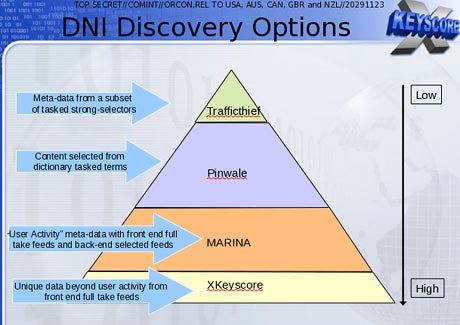
\includegraphics[scale=0.65]{KS10-001.png} 
\caption{{\lt Miscellaneous D.N.I (Digital Network Intelligence - intelligence collected by Internet traffic) Software used be NSA and Five Eyes}}
\end{figure}

	
\item[{\lt iv)}] Ασφάλεια {\lt OTP}

	Το {\lt OTP} δεν παραμένει ασφαλές αν χρησιμοποιηθεί το ίδιο κλειδί περισσότερες από μία φορές. Αυτό ισχύει για τους παρακάτω λόγους.\\

	Αρχικά, σε περίπτωση που ο επιτηθέμενος, με κάποιον τρόπο, αποκτήσει ένα από τα δύο {\lt plaintext}, μπορεί να αποκρυπτογραφίσει και το άλλο χρησιμοποιώντας το ίδιο κλειδί.\\

	Ακόμη, αν ο επιτιθέμενος αποκτήσει πολλά μηνύματα που έχουν κρυπτογραφηθεί με το ίδιο κλειδί, μπορεί να επιχειρήσει την επίθεση που χρησιμοποιείται και στο κρυπτοσύστημα μετατόπισης. Δηλαδή, μπορεί να βρεί τις συχνότητες εμφάνισης χαρακτήρων και να επιχειρήσει να βρεί το κλειδί. Αυτό ισχύει διότι, χρησιμοποιώντας το ίδιο κλειδί, οι χαρακτήρες των δύο μηνυμάτων που βρίσκονται στις ίδιες θέσεις, έχουν υποστεί την ίδια μετατόπιση.\\

	Τέλος, ο {\lt OTP} είναι ασφαλής ακόμα και ενάντια σε {\lt brute force attacks} καθώς, όλες οι πιθανές περιπτώσεις κλειδιού θα οδηγήσουν σε όλα τα πιθανά μηνύματα. Έτσι, ο {\lt attacker} δεν μπορεί να γνωρίζει το πραγματικό περιεχόμενο. Αν όμως χρησιμοποιηθεί το ίδιο κλειδί, μπορεί να διαπιστωθεί αν ένα πιθανό κλειδί οδηγεί σε πραγματικό κείμενο και για τα δύο κρυπτομηνύματα. Αυτό, αν και δεν δίνει μεγάλο προβάδισμα στον επιτιθέμενο, αυξάνει, έστω και λίγο, τις πιθανότητες να βρεί το αρχικό μήνυμα.

	\item[{\lt v)}] {\lt GCM}

	To {\lt GCM (Galois Counter Mode)} είναι μία ιδιαίτερα δημοφιλής κατάσταση λειτουργίας για συμμετρικά κρυπτοσυστήματα τμήματος. Σημαντικό χαρακτηριστικό του είναι πως, εκτός από κρυπτογράφηση, προσφέρει και αυθεντικοποίηση. \\

	\subsection*{Περιγραφή αλγορίθμου}
	Η λειτουργία κρυπτογράφησης του {\lt GCM} βασίσεται στο κλασσικό {\lt counter mode} το οποίο σημαίνει:
	\begin{itemize}
		\item Το αρχικό κείμενο σπάει σε {\lt blocks} των 128 {\lt bits}
		\item Δημιουργείται ένας {\lt counter} που παίρνει τιμές μέχρι το πλήθος των {\lt block} του αρχικού κειμένου
		\item Ένα τυχαίο {\lt IV} συνενώνεται με έναν {\lt counter} και κρυπτογραφείται με έναν συμμετρικό αλγόριθμο κρυπτογράφησης τμήματος (π.χ. {\lt AES DES})
		\item Tο αποτέλεσμα γίνεται {\lt XOR} με το αντίστοιχο {\lt block} του αρχικού κειμένου
	\end{itemize}

	Αυτή η κατάσταση λειτουργίας είναι ευπαθής σε περιπτώσεις όπου κάποιος τρίτος μπορεί να προκαλέσει αλλαγές στο κρυπτογραφημένο κείμενο κατά την ανταλλαγή του. Για να εξασφαλίσουμε ακεραιότητα και αυθεντικοποίηση, πρέπει να χρησιμοποιηθεί μία {\lt MAC} επί του κρυπτογραφημένου κειμένου και του {\lt IV}.

	Για να επιτευχθεί αυτό χρησιμοποιείται η {\lt GMAC}, δηλαδή μία {\lt MAC} που χρησιμοποιεί πολλαπλασιασμό στο $GF(2^{128})$. Αναλυτικότερα:
	\begin{itemize}
		\item Το αποτέλεσμα κρυπτογράφησης από του πρώτου {\lt block} περνά από πολλαπλασιασμό σε $GF(2^{128})$
		\item Το αποτέλεσμα κρυπτογράφησης από το επόμενο {\lt block} γίνεται {\lt XOR} με το αποτέλεσμα του προηγούμενου βήματος και περνά από πολλαπλασιασμό σε $GF(2^{128})$
		\item Όταν γίνουν πολλαπλασιασμοί και {\lt XOR} σε όλα τα {\lt block}, το αποτέλεσμα, γίνεται {\lt XOR} με το μήκος του κειμένου και περνά από έναν πολλαπλασιασμό
		\item Το τυχαίο {\lt IV} συνενωμένο με τον {\lt counter 0} περνά από πολλαπλασιασμό σε $GF(2^{128})$ και γίνεται {\lt XOR} με το προηγούμενο βήμα.
	\end{itemize}
	Το αποτέλεσμα είναι ένα {\lt TAG} που συνενώνεται με το κρυπτογραφημένο κείμενο.

	Το {\lt GCM} έχει μία ακόμα πολύ σημαντική δυνατότητα. Μπορεί να εξασφαλίσει την ακεραιότητα παραπάνω δεδομένων. Για παράδειγμα, δεδομένα που έχουν σχέση με τα πακέτα που ανταλλάσσονται, αν πρόκειται για επικοινωνία μέσω διαδικτύου. Αυτά τα στοιχεία περνούν από πολλαπλασιασμό σε $GF(2^{128})$ και στη συνέχεια γίνονται {\lt XOR} με το πρώτο {\lt block} κρυπτογραφημένου κειμένου. Η διαδικασία συνεχίζεται όπως περιγράφεται παραπάνω.
	\begin{figure}[!ht]
	\centering
	\includegraphics[scale=0.4]{gcm.png}
	\caption{Αλυσίδα {\lt GMAC}}
	\end{figure}

	\subsection*{Πολλαπλασιασμός σε $GF(2^{128})$}
	Η διαδικασία που αναφέρθηκε ως πολλαπλασιασμός σε $GF(2^{128})$ αναλύεται σε μεγαλύτερη λεπτομέρεια παρακάτω. Ουσιαστικά πρόκειται για πολλαπλασιασμό πολυωνύμων.

	Αρχικά επιλέγεται ένα δεύτερο κλειδί των 128 {\lt bits}. Το κλειδί αυτό, καθώς και τα 128 {\lt bits} που δίνονται σε κάθε βήμα του {\lt GMAC} αναπαριστούν πολυώνυμα που ανήκουν στο $GF(2^{128})$, δηλαδή πολυώνυμα μέχρι και 127ου βαθμού. Αυτά τα δύο πολυώνυμα πολλαπλασιάζονται μεταξύ τους και το αποτέλεσμα που προκύπτει, επιστρέφεται ως ακολουθία των 128 {\lt bits}.

	Επομένως, όπως βλεπουμε, για την χρήση της κατάστασης λειτουργίας {\lt GCM}, απαιτούνται 2 κλειδιά των 128 {\lt bit}:
	\begin{itemize}
		\item Ένα για την κρυπτογράφηση με συμμετρικό αλγόριθμο τμήματος
		\item Ένα για τον πολλαπλασιασμό σε $GF(2^{128})$
	\end{itemize}
	
\end{itemize}

\newpage


% ===== Θέμα 2 =====
\section*{Θέμα 2}

\tabΗ άσκηση αυτή είχε ως στόχο την δημιουργία του αλγορίθμου κρυπτογράφησης {\lt RC4} και την κρυπτογράφηση ενός μηνύματος. Επιπλέον, δημιουργήθηκε μια συνάρτηση αποκρυπτογράφησης για τον έλεγχο της επιτυχής κρυπτογράφησης. Περιληπτικά, τα βήματα που εκτελέστηκαν ήταν τα εξής:
\begin{enumerate}

\item Μετατροπή του κλειδιού "{\lt MATRIX}" σε {\lt bits} με την δοσμένη 5-{\lt bit} κωδικοποίηση και δημιουργία ενός πίνακα {\lt S} μεγέθους 256 με ανακατεμένες τιμές από 0 εώς 255 με βάση τα {\lt bits} των γραμμάτων του μηνύματος.

\item Δημιουργία μιας κρυπτοροής Κ από {\lt bits}, με βάση συγκεκριμένους τύπους του {\lt RC4} που εμπλέκουν τον παραπάνω πίνακα {\lt S} με παρόμοιες τιμές.

\item Μετατροπή της κρυπτοροής Κ σε {\lt bits}, εκτέλεσης πράξης {\lt XOR} μεταξύ αυτής και του μηνύματος και μετατροπή σε χαρακτήρες με βάση την 5-{\lt bit} κωδικοποίηση.

\item Αποκρυπτογράφηση του πλέον κρυπτογραφημένου μηνύματος με το κλειδί ακολουθώντας παρομοίως την παραπάνω διαδικασία. \\

\end{enumerate}


Τα αποτελέσματα του προγράμματος είναι το κρυπτογραφημένο μήνυμα: \\
\textit{{\lt -sc-od(xumaj?!?gd?(a)hj-xyslufm}} \\
και το αποκρυπτογραφημένο (δηλαδή το αρχικό) μήνυμα: \\
\textit{{\lt neversendahumantodoamachinesjob}}



\newpage


% ===== Θέμα 3 =====
\section*{Θέμα 3}
\tabΑρχικά έγινε προσπάθεια εύρεσης του μήκους του κλειδιού που χρησιμοποιήθηκε για την κρυπτογράφηση.
Χρησιμοποιώντας τον δείκτη σύμπτωσης ({\lt Index of Coincidence}) που υλοποιήθηκε σε {\lt Python} και έτσι βρέθηκε
με μεγάλη βεβαιότητα ότι το μήκος του κλειδιού είναι 7 χαρακτήρες ({\lt IC} = 0.06722).
\\
Έτσι το κείμενο διασπάστηκε σε 7 στήλες έτσι ώστε να ισχύει η ίδια μετατόπιση σε κάθε στήλη. Κάνοντας ανάλυση συχνοτήτων
των χαρακτήρων κάθε στήλης, βρέθηκαν οι πιο συχνοί χαρακτήρες κάθε στήλης. Αυτοί είναι:

{\lt
\begin{itemize}
	\item I
	\item Q
	\item T
	\item I
	\item V
	\item S
	\item V
\end{itemize}
}

Αν θεωρηθεί ότι αυτοί οι χαρακτήρες αντιστοιχούν στο {\lt E} (που είναι το γράμμα με την υψηλότερη συχνότητα εμφάνισης), τα
κλειδιά που προκύπτουν σε κάθε στήλη είναι:

\begin{itemize}
	\item Μετατόπιση 4 άρα κλειδί {\lt E}
	\item Μετατόπιση 12 άρα κλειδί {\lt M}
	\item Μετατόπιση 15 άρα κλειδί {\lt P}
	\item Μετατόπιση 4 άρα κλειδί {\lt E}
	\item Μετατόπιση 17 άρα κλειδί {\lt R}
	\item Μετατόπιση 14 άρα κλειδί {\lt O}
	\item Μετατόπιση 17 άρα κλειδί {\lt R}
\end{itemize}

Παρατηρείται ότι σχηματίζουν τη λέξη {\lt EMPEROR} και έτσι φαίνεται πως βρέθηκε το σωστό κλειδί. Με αποκρυπτογράφηση του
μηνύματος με αυτό το κλειδί, προκύπτει το σωστό κείμενο

Αν το κλειδί που προέκυπτε από την παραπάνω ανάλυση ήταν λάθος, θα δοκιμάζονταν άλλοι συνδιασμοί βρίσκοντας τα δεύτερα πιο συχνά εμφανιζόμενα γράμματα κλπ.




\newpage


% ===== Θέμα 4 =====
\section*{Θέμα 4}
\tabΕφόσον χρησιμοποιείται το σύστημα μετατόπισης, τα πιθανά κλειδιά είναι μόλις 23. Επομένως, με επίθεση ωμής βίας μπορούν να
δοκιμαστούν όλα τα πιθανά κλειδιά. Βλέποντας τα αποτελέσματα, παρατηρείται ότι το κείμενο που προκύπτει χρησιμοποιώντας το κλειδί 3 είναι:\\
ΜΗΔΕΙΣΑΓΕΩΜΕΤΡΗΤΟΣΕΙΣΙΤΩΜΟΥΤΗΝΣΤΕΓΗΝ.\\
Αντίθετως, το κείμενα που προκύπτουν από τα υπόλοιπα κλειδιά δεν έχουν κάποιο νόημα. Έτσι έχουμε βρεθεί ότι
το κλειδί είναι 3 και το κείμενο ΜΗΔΕΙΣ ΑΓΕΩΜΕΤΡΗΤΟΣ ΕΙΣΙΤΩ ΜΟΥ ΤΗΝ ΣΤΕΓΗΝ.






% ===== Θέμα 5 =====
\section*{Θέμα 5}

\tabΣτο θέμα αυτό εξετάστηκε το ποσοστό του {\lt avalanche effect} στον {\lt AES} μεταξύ διαφόρων ζευγαριών μηνυμάτων που διέφεραν μεταξύ τους σε ένα {\lt bit}. \\
Συγκεκριμένα, 32 λέξεις/φράσεις μήκους 16 χαρακτήρων/{\lt bytes} μετράπηκαν σε δεκαεξαδικό και ύστερα σε δυαδικά ψηφία και τροποιήθηκε ένα {\lt bit} από την σειρά αυτή δημιουργώντας ένα σχεδόν ίδιο μήνυμα.
Στην συνέχεια, τα αρχικα και τα τροποποιημένα μηνύματα κρυπτογραφήθηκαν με τον {\lt AES} σε {\lt ECB mode} και {\lt CBC mode} για να εξαταστούν οι διαφορές σε επίπεδο {\lt bit} του κρυπτογραφημένου αρχικού μηνύματος με το κρυπτογραφημένο τροποποιημένο μήνυμα. \\
Τα αποτελέσματα του προγράμματος σε κάθε εκτέλεση διαφέρουν σε έναν μικρό βαθμό καθώς επιλέγεται κάθε φόρα διαφορετικό {\lt bit} του μηνύματος για τροποποίηση. 
Σε γενικές γραμμές, βρέθηκε ότι το ποσοστό των μεταλλαγμένων {\lt bits} σε {\lt ECB mode} αλλά και σε {\lt CBC mode} ήταν εντός του διαστήματος 49-51\% ικανοποιώντας το κριτήριο του {\lt avalanache effect} (50\%) για την έξοδο του κρυπτοσυστήματος να είναι ανεξάρτητη από την είσοδό του.




\newpage
% ===== Θέμα 6 =====
\section*{Θέμα 6}

\tabΗ μέθοδος που εκτελέστηκε για την αποκρυπτογράφηση του μηνύματος βασίστηκε στην δημιουργία τριών διαφορετικών μηνυμάτων που προέκυψαν αποκρυπτογραφώντας κάθε φόρα το μήνυμα με ένα από τα γράμματα {\lt K}, {\lt E} και {\lt Y}. 
Αναλυτικότερα, τα μηνύματα αυτά μπορούν να προκύψουν είτε από συνεχείς αλγεβρικές πράξεις με βάση τον τύπο $ X  Μod 26 - S_{i} $ όπου $S_{i} : i = {K, E, Y} $ είτε με την χρήση του παρακάτω δίσκου.

\centerline{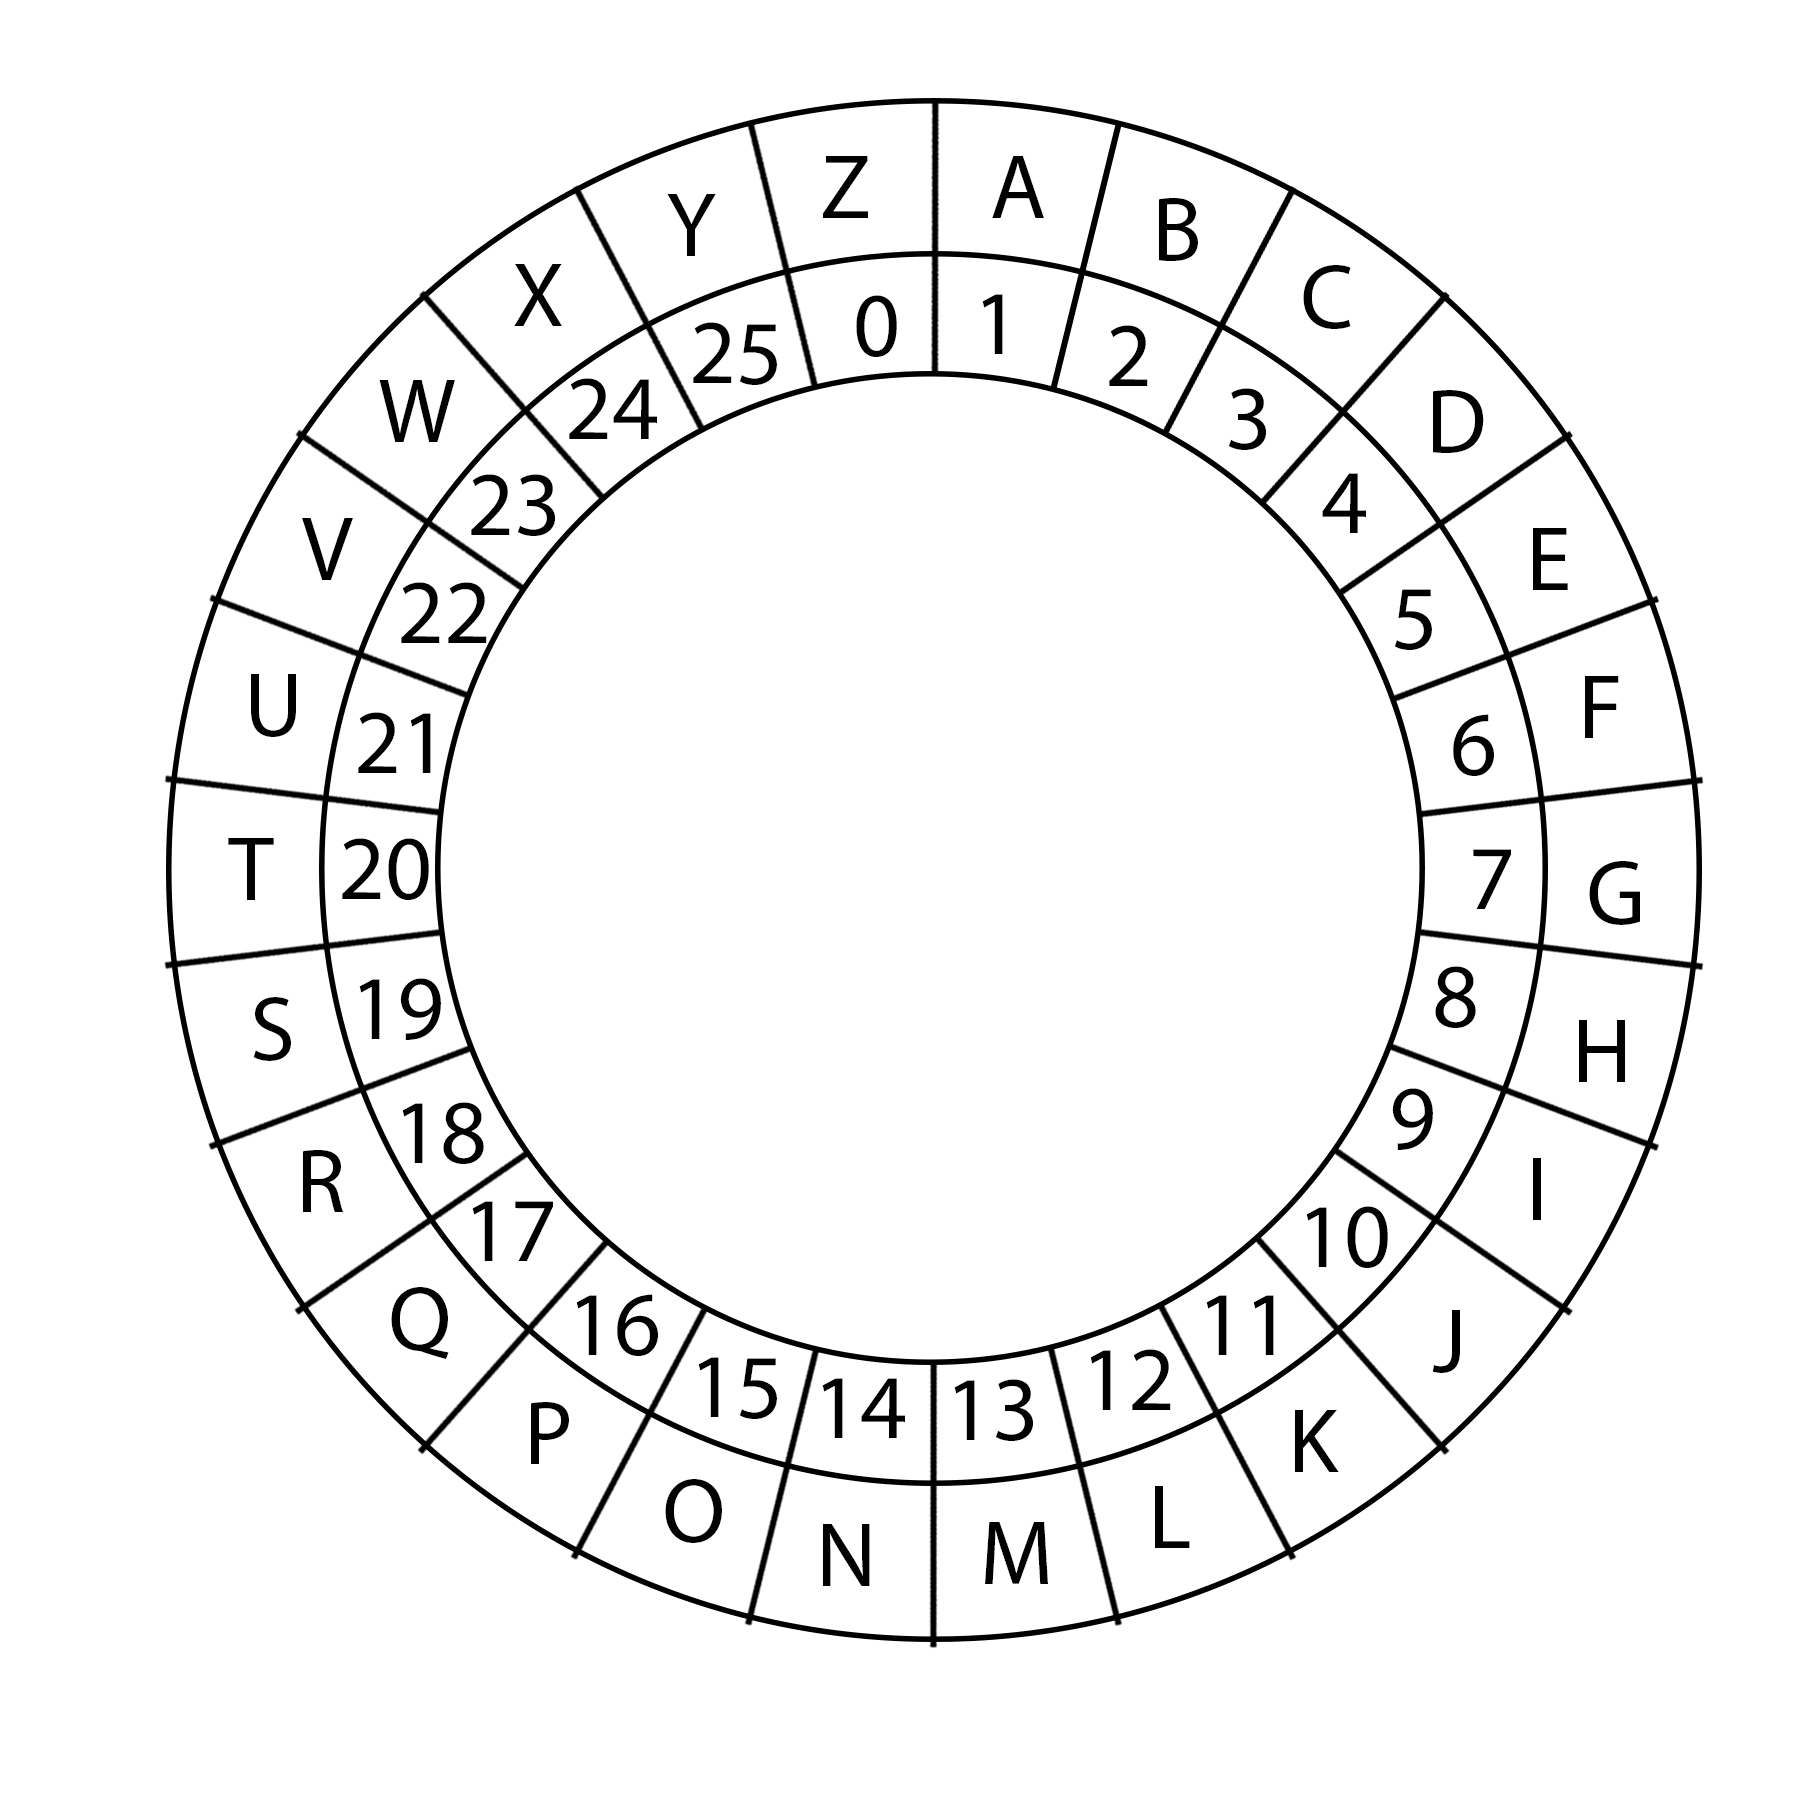
\includegraphics[scale=0.35]{disk.png}} 
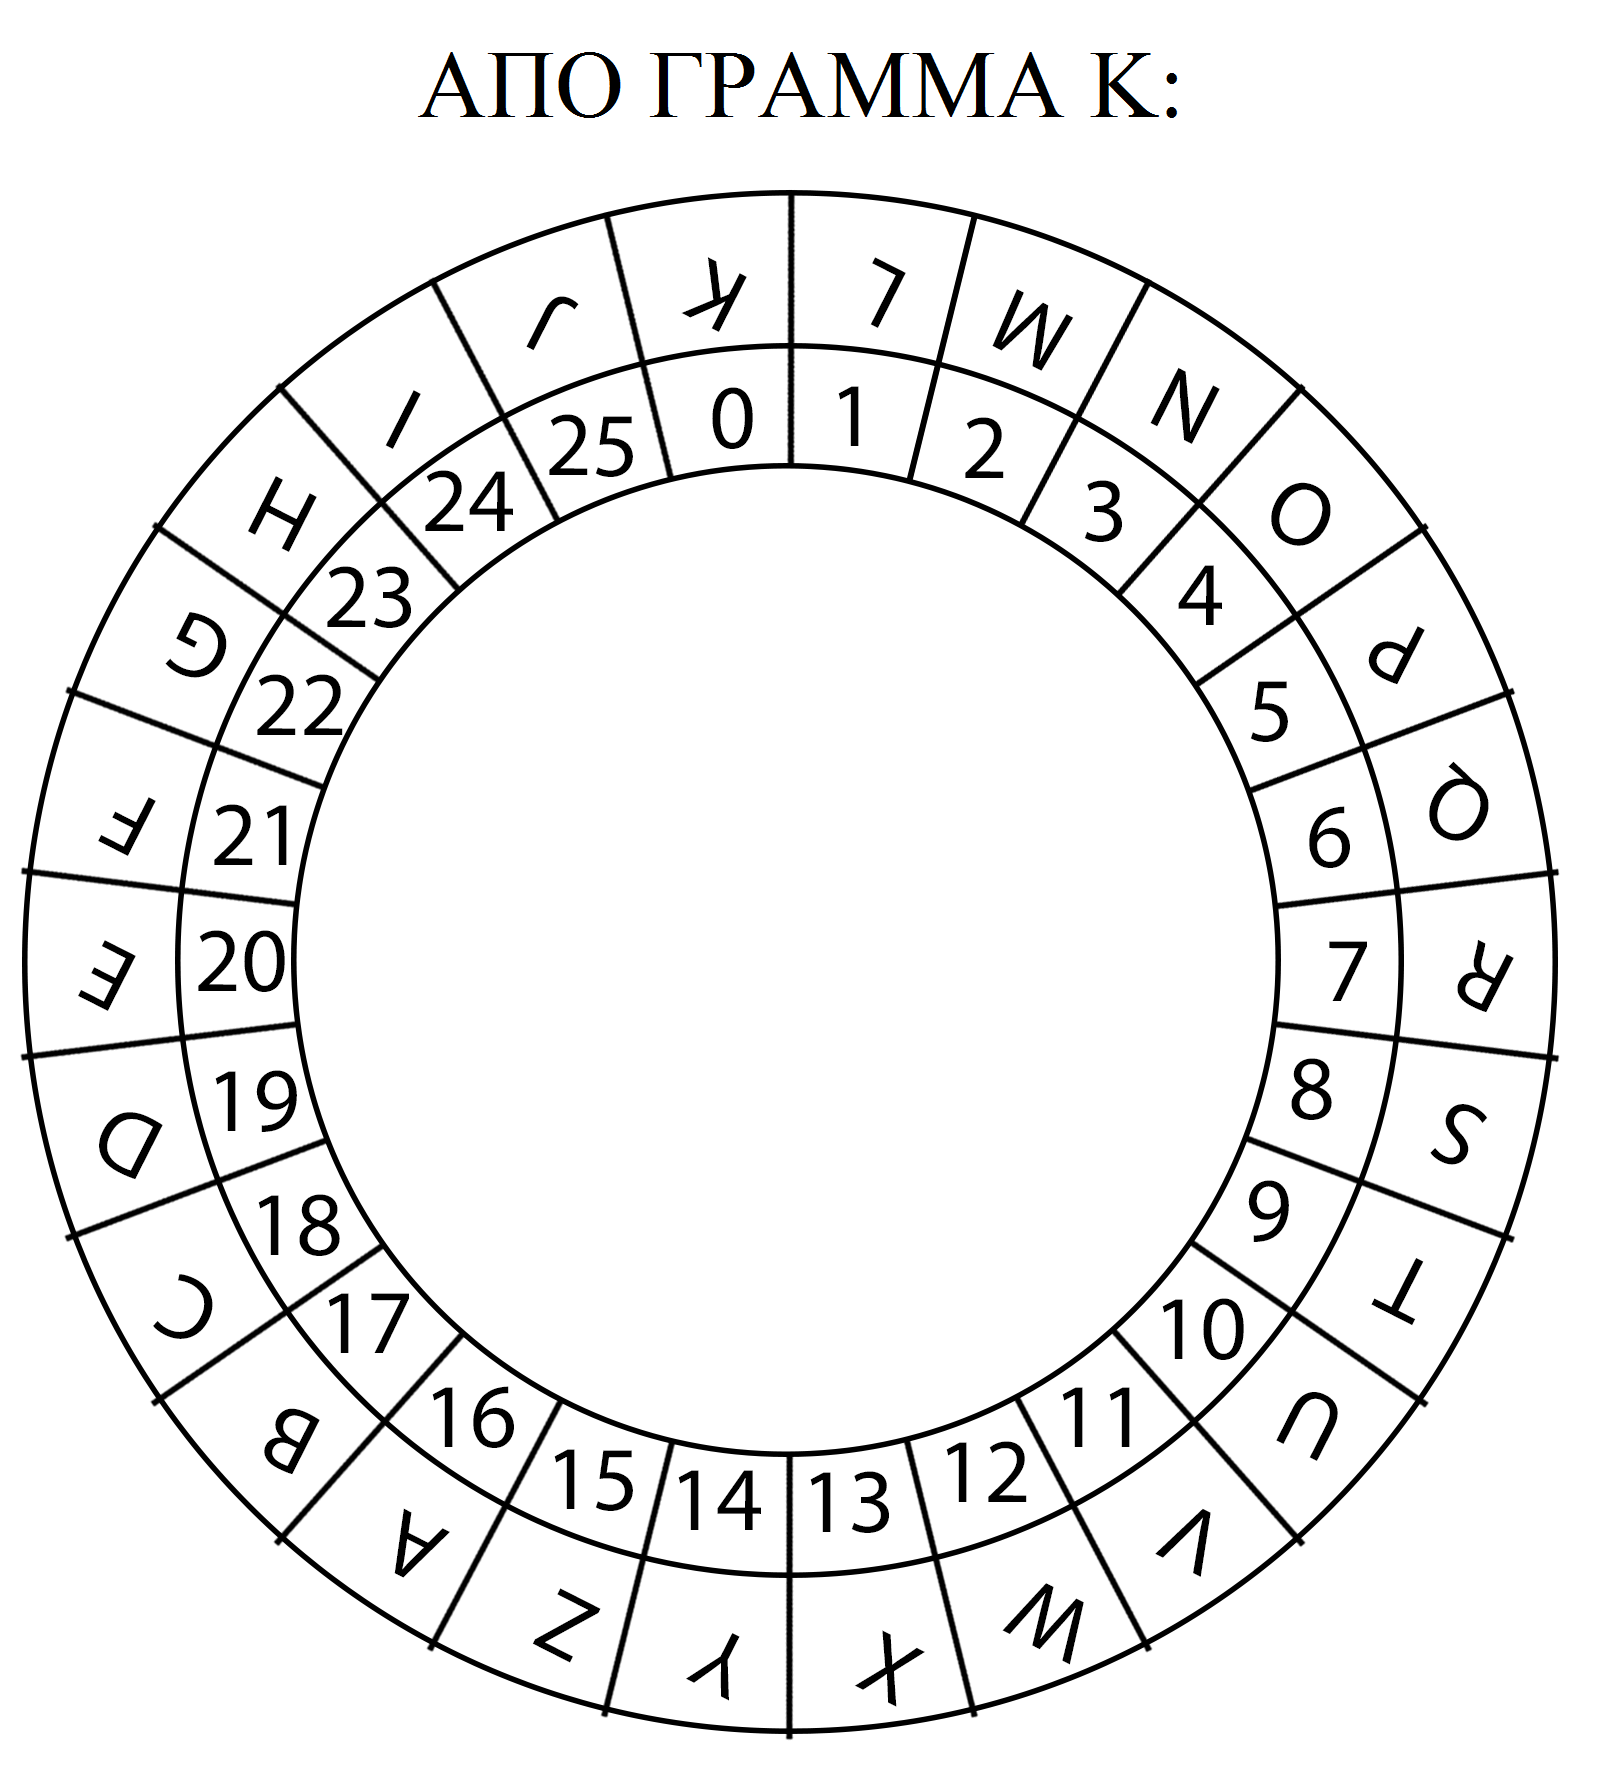
\includegraphics[scale=0.08]{diskwithk.png}  
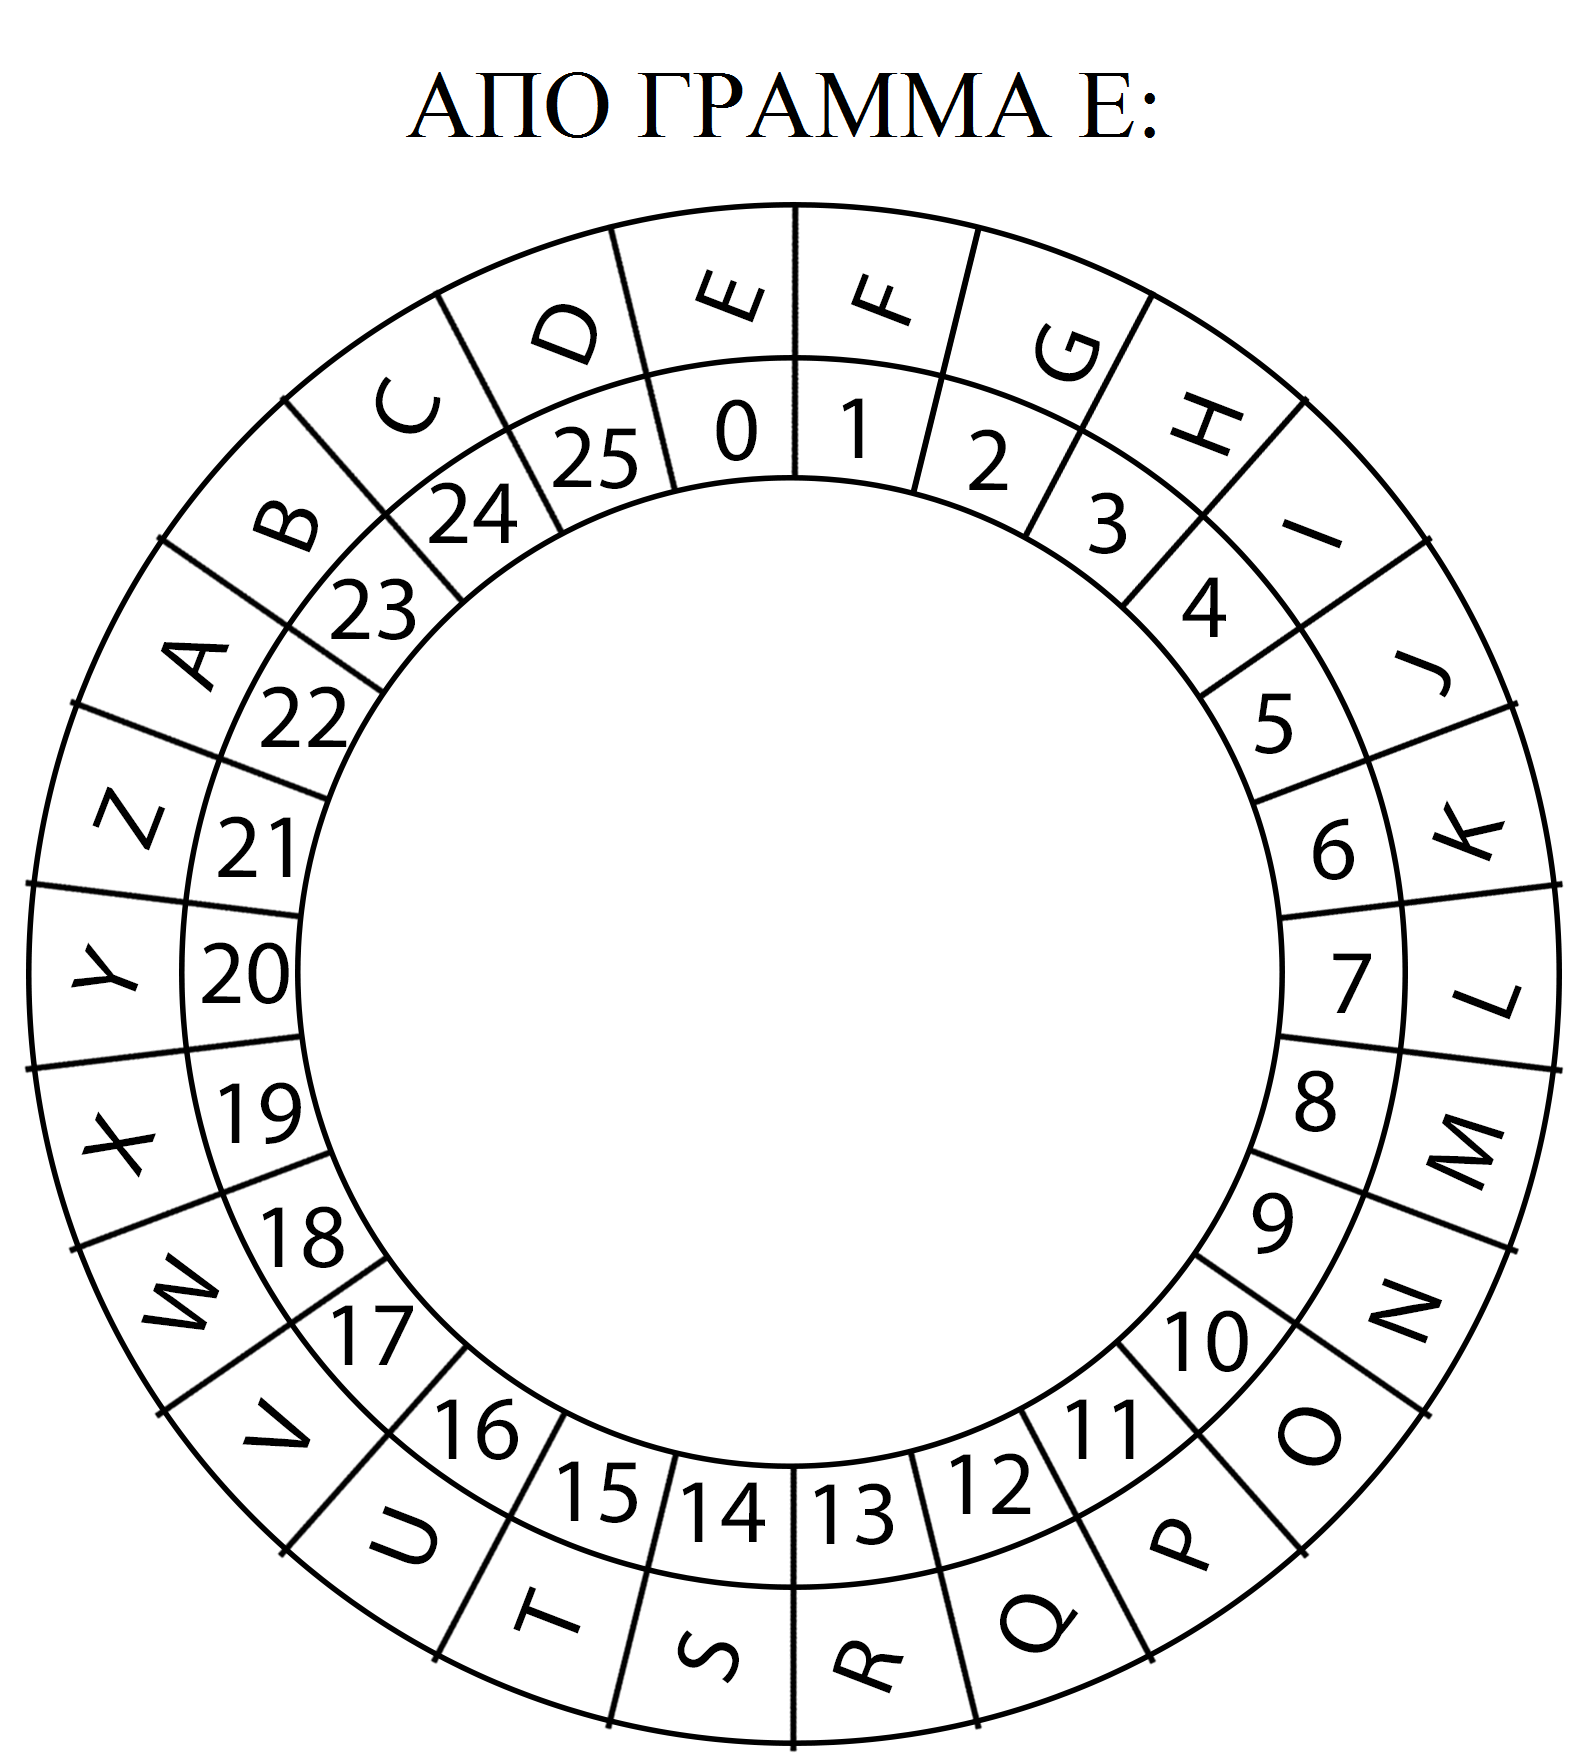
\includegraphics[scale=0.08]{diskwithe.png}   
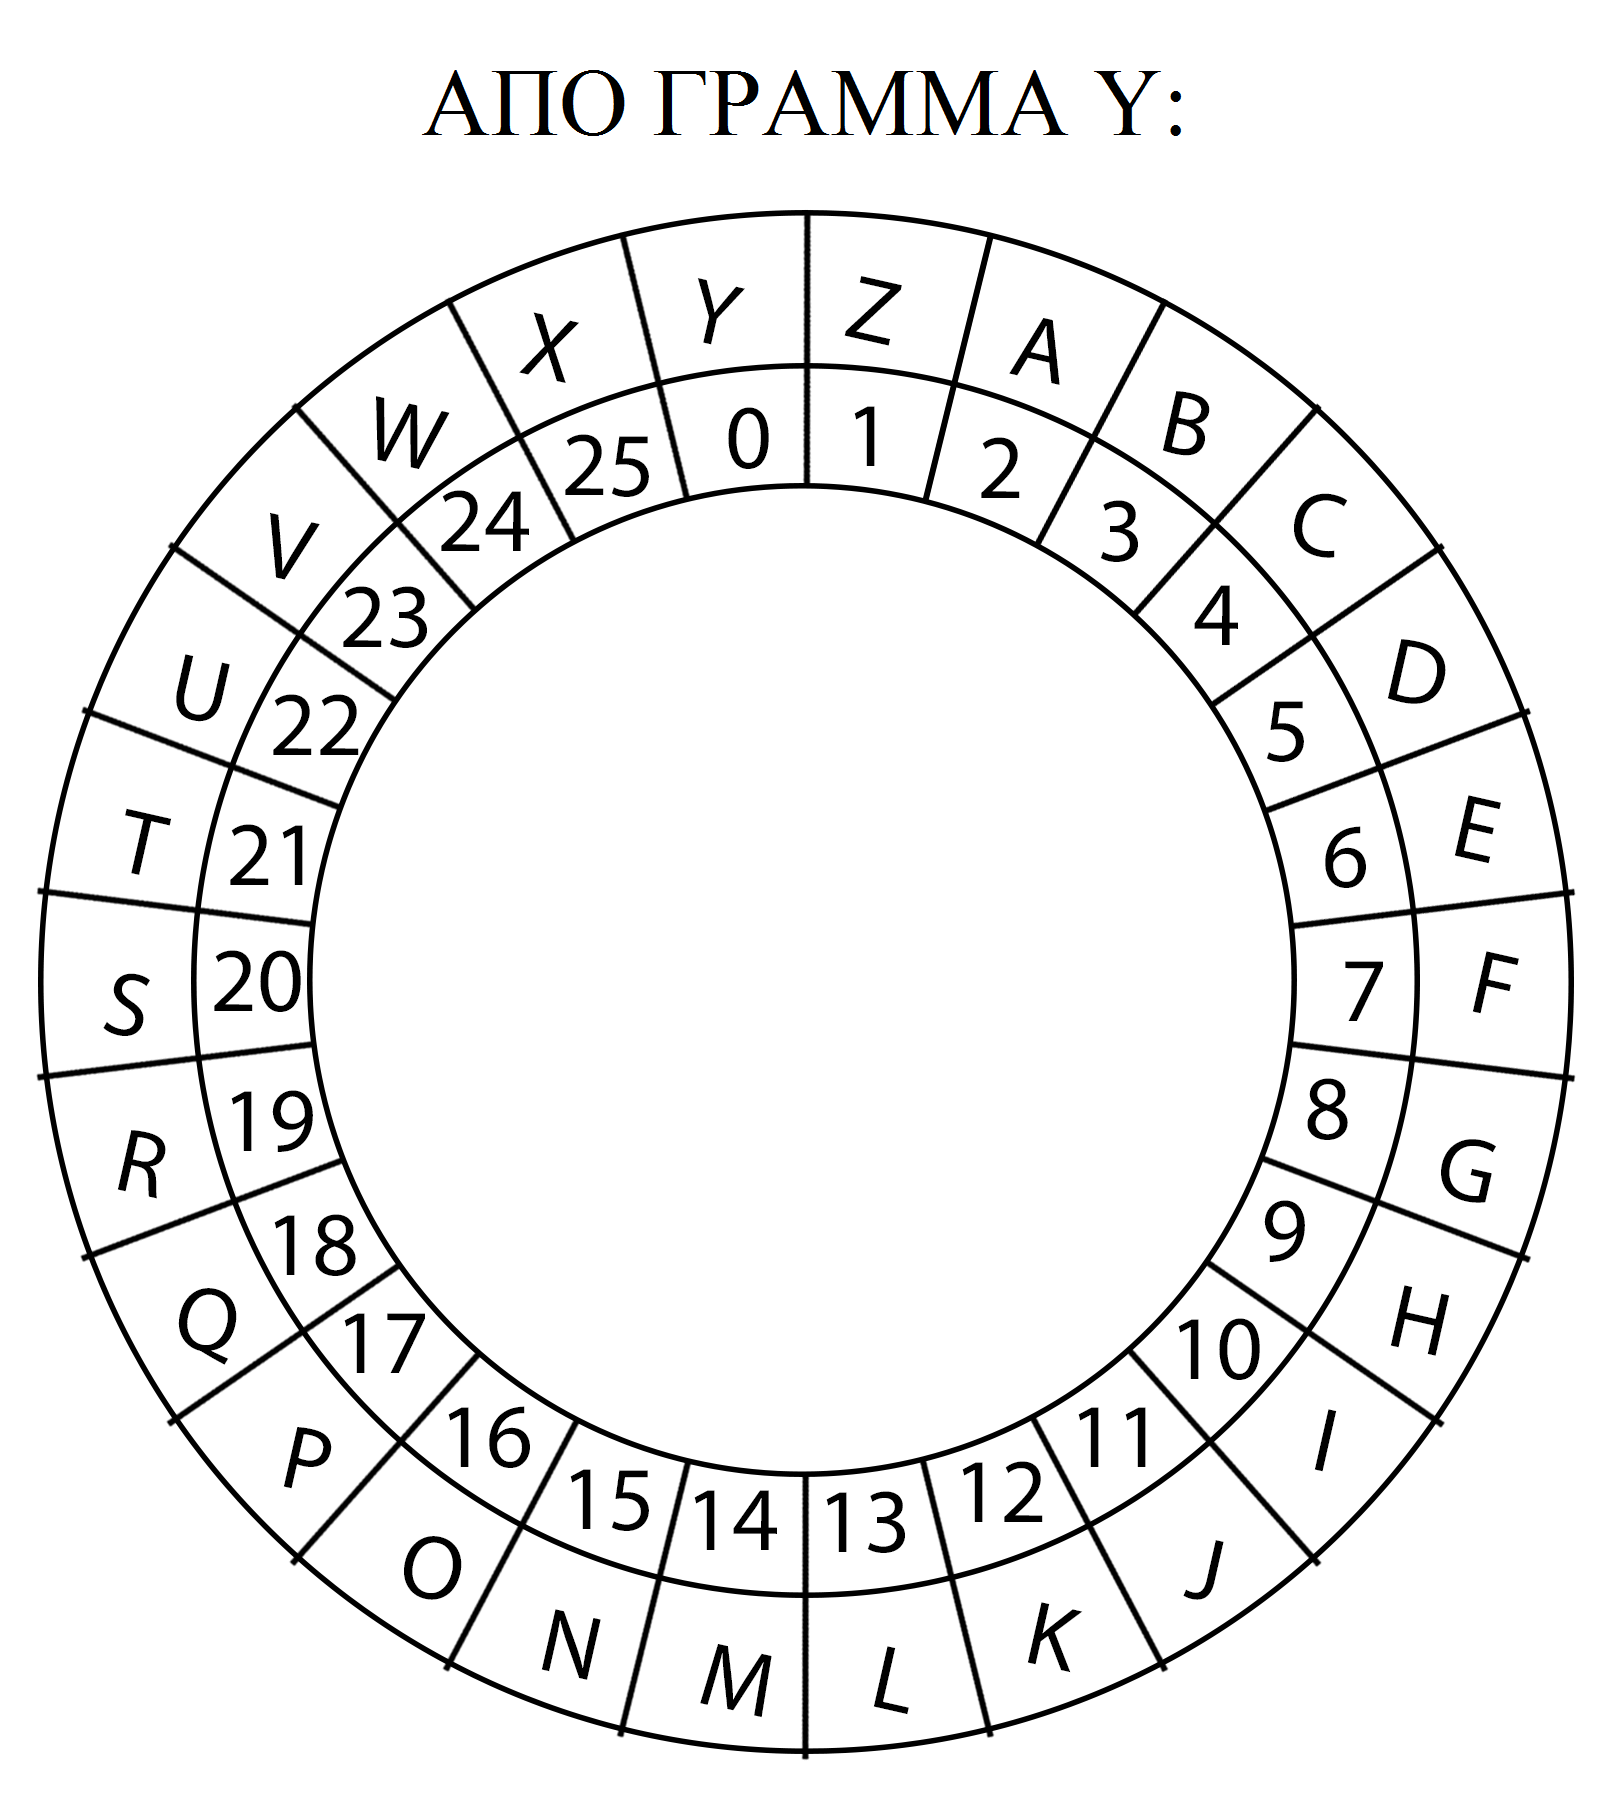
\includegraphics[scale=0.08]{diskwithy.png} 
 
Ο δίσκος αυτός αναπαριστά το αλφάβητο σε κυκλική μορφή για την διευκόλυνση της εύρεσης του αποτελσματος του {\lt mod26}. 
Για παράδειγμα, για την αποκρυπτογράφηση ενός γράμματος (π.χ το Α) με βάση το γράμμα Κ , δημιουργείται αρχικά ένας νέος δίσκος στον οποίο ο εξωτερικός δαχτύλιος έχει περιστραφεί έτσι ώστε το Κ να βρίσκεται πάνω από τον αριθμό 0. Στην συνέχεια, σημειώνεται ο αριθμός της θέση στην οποία το γράμμα Α βρίσκεται στον νέο δίσκο και επιστρέφοντας στον παλιό δίσκο σε εκείνη την θέση βρίσκεται το αποκρυπτογραφημένο γράμμα, σε αυτήν την περίπτωση το {\lt P}.

Τελικά, χρησιμοποιώντας την παρακάτω συμβολοσείρα με την παραπάνω μέθοδο και με την δημιουργία των τριών αυτών συμβολοσειρών η εύρεση του μηνύματος ήταν σχετικά εύκολη. Επιλέγοντας, διασθητικά, γράμματα από κάθε συμβολοσειρά ώστε να σχηματίζονται υπαρκτές λέξεις βρέθηκε η παρακάτω φράση. \\
Είσοδος: {\lt AJZBPMDLHYDBTSMFDXTQJ} \\
Έξοδος:  {\lt PEACEBEGINSWITHASMILE (Peace begins with a smile)}



\newpage


% ===== Θέμα 7 =====
\section*{Θέμα 7}
\tabΧρησιμοποιήθηκε επίθεση ωμής βίας, δηλαδή δοκιμάστηκαν ως κλειδιά όλες οι λέξεις που βρίσκονται στο {\lt english.txt}. Μετά απο αρκετές προσπάθειες
βρέθηκε το κλειδί: {\lt secret}.



% ===== Θέμα 8 =====
\section*{Θέμα 8}
Χρησιμοποιήθηκε επίθεση ωμής βίας, δηλαδή δοκιμάστηκαν ως κλειδιά όλοι οι εξαψήφιοι ακέραιοι. Για να βρεθεί ποιός από τους αριθμούς είναι ο κωδικός, χρησιμοποιήθηκε η εξής μεθοδολογία:\\

Αρχικά, ο κωδικός αποθηκεύεται μετά από {\lt hashing} με {\lt sha512} (\$6\$) και {\lt salt} {\lt kHnyu3Ni} όπως δίνονται στο το {\lt /etc/shadow}. Αν το αποτέλεσμα του αλγορίθμου είναι ίδιο με το {\lt hash} που μας δίνεται, τότε ο κωδικός έχει βρεθεί.\\

Έτσι βρέθηκε ότι το {\lt password} είναι: 676767



\newpage


% ===== Θέμα 9 =====
\section*{Θέμα 9}
\subsection*{{\lt (i)}}
Έστω $K$ το {\lt keystream} που χρησιμοποιήθηκε για την κρυπτογράφηση.\\
Έστω $C$ το κρυπτογραφημένο κείμενο.\\
Για να βρεθεί το αρχικό κείμενο ακολουθήθηκε η παρακάτω διαδικασία:\\

Πρώτα, χρησιμοποιώντας το {\lt known plaintext} $ab$ για το κρυπτογραφημένο $sq$, μπορούν να βρεθούν τα {\lt bits} 10-19 του $Κ$.
Αυτό γίνεται κάνοντας {\lt XOR} μεταξύ των 5-{\lt bit} κωδικοποιήσεων των $ab$ και $sq$.

Γνωρίζουμε πως τα {\lt bits} $Κ[10:20]$ που βρέθηκαν, είναι μία ανεστραμμένη κατάσταση του {\lt LFSR} (λόγω της ιδιότητας του {\lt LFSR} να βγάζει
αντίστροφα τα {\lt bits} των καταστάσεων μέσα στο $K$). Συγκεκριμένα γνωρίζουμε ότι τα {\lt bits} $Κ[10:20]$ μας δίνουν την 10 κατάσταση του {\lt LFSR}.\\

\noindent Έστω $S$ η αντεστραμμένη ακολουθία των {\lt bits} 10-19\\

Για να βρούμε το πλήρες {\lt keystream} μπορούν να ακολουθηθούν δύο μεθοδολογίες:

\begin{itemize}
\item Αντίστροφο {\lt LFSR} ξεκινώντας από την κατάσταση 10 μέχρι να βρεθεί το {\lt seed} (κατάσταση 0)
\item Εκτέλεση του {\lt LFSR} με κλειδί τo $S$ και χρησιμοποίηση μόνο ενός τμήματος του {\lt stream}
\end{itemize}

Για λόγους ευκολίας υλοποίησης, χρησιμοποιήθηκε η δεύτερη μεθοδολογία. Αναλυτικότερα, το $Κ$ είναι το τμήμα του {\lt stream} που έχει:\\
\begin{itemize}
\item Έναρξη: 1023 - 10 = 1013 \\(Περίοδος του {\lt LFSR} - μετατόπιση επειδή δόθηκε ως κλειδί η 10η κατάσταση)\\
\item Μήκος: {\lt len(Ciphertext)} * 5 \\(Αριθμός χαρακτήρων του κρυπτογραφημένου * 5 {\lt bit} ανά χαρακτήρα)\\
\end{itemize}

Έτσι προκύπτει το $K$. Κάνοντας {\lt XOR} μεταξύ του $K$ και του $C$, γίνεται γνωστό το αρχικό μήνυμα.

\newpage
\subsection*{{\lt (ii)}}
Έστω $K1$ το {\lt stream} που προκύπτει από το {\lt LFSR-10}.\\
Έστω $K2$ το {\lt stream} που προκύπτει από το {\lt LFSR-16}.\\
Έστω $K3$ το {\lt keystream} που προκύπτει από το {\lt XOR} των $K1$ και $K2$.\\

Αρχικά, δίνονται τα {\lt bits} 10-29 με παρόμοιο τρόπο όπως στο προηγούμενο υποερώτημα. Επίσης, με {\lt brute force} στο {\lt seed} του {\lt LFSR-10}, μπορούν να βρεθούν όλα τα πιθανά $K1$.\\

Κάνοντας {\lt XOR} μεταξύ του γνωστού τμήματος του $K3$ και κάθε πιθανού $K1$, είναι δυνατό να βρεθούν 20 {\lt bits} του $K2$. Αυτά, κάνοντας αντίστροφο {\lt LFSR}, μπορούν να χρησιμοποιηθούν για την εύρεση του {\lt seed}.\\

Επομένως έχουν προκύψει 1024 ζεύγη {\lt seed} για τα δύο {\lt LFSR}. Άρα μπορούν να βρεθούν 1024 πιθανά κείμενα τα οποία αποτελούν το αρχικό κείμενο.\\

Για τον περιορισμό των πιθανών αποτελεσμάτων, χρησιμοποιήθηκε η παρακάτω τεχνική:
\begin{itemize}
	\item Τα γνωστά {\lt bits} 10-25 του $K2$ χρησιμοποιούνται για την εύρεση του 2ου {\lt seed}.
	\item Μετά την εύρεση του πιθανών {\lt seed} και $Κ2$, γίνεται έλεγχος εάν τα {\lt bits} 26-29 του $K2$ είναι ίδια με τα γνωστά {\lt bits}. Αν ναι, τότε αυτό το {\lt stream} θεωρείται έγκυρο.
\end{itemize}

Τελικά, μετά την εκτέλεση του αλγορίθμου, προέκυψαν περίπου 60 πιθανές προτάσεις από τις οποίες αναγνωρίστηκε η παρακάτω:\\
{\lt alwaysforgiveyourenemies.nothingannoysthemsomuch}





\end{document}
